\chapter{Исследовательская часть}

В данном разделе будут приведены примеры работы программ, постановка эксперимента и сравнительный анализ алгоритмов на основе полученных данных.

\section{Технические характеристики}

Технические характеристики устройства, на котором выполнялось исследование.

\begin{enumerate}
	\item Операционная система: Windows 10 Корпоративная, Версия	21H1, Сборка ОС 19043.2006.
	\item Оперативная память: 8 ГБ.
	\item Процессор: AMD Ryzen 5 4600H с видеокартой Radeon Graphics \\3.00 ГГц \cite{processor}.
\end{enumerate}

Исследование проводилось на ноутбуке, включенном в сеть электропитания. Во время исследования ноутбук был нагружен только встроенными приложениями окружения, а также непосредственно системой.

\section{Демонстрация работы программы}

На рисунках \ref{fig:demographics}, \ref{fig:smoke}, \ref{fig:democonsole}, представлены результат работы алгоритма обратной трассировки лучей.

\captionsetup{justification=centering, singlelinecheck=false}
\begin{figure}[H]
	\centering
	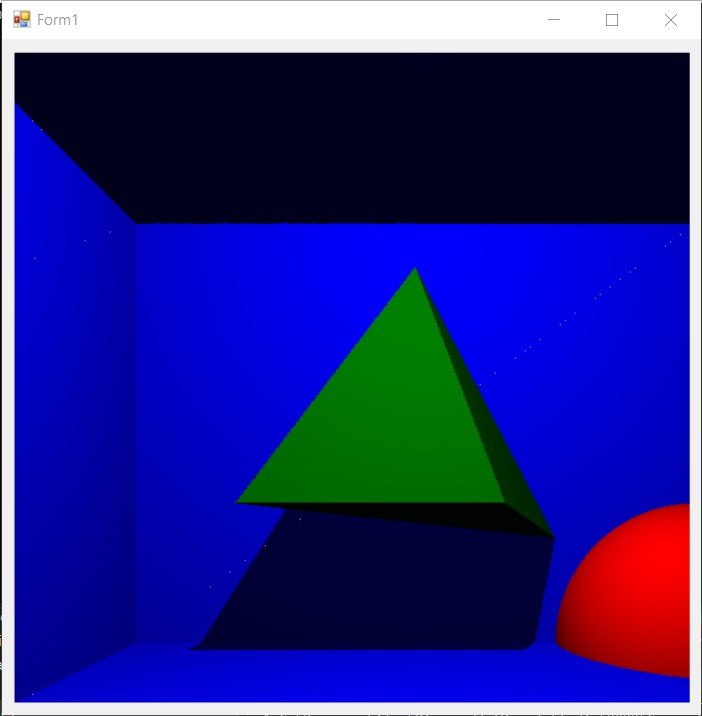
\includegraphics[width=1\linewidth]{inc/img/demographics}
	\caption{Демонстрация работы программы в графическом интерфейсе без дыма}
	\label{fig:demographics}
\end{figure}
\begin{figure}[H]
	\centering
	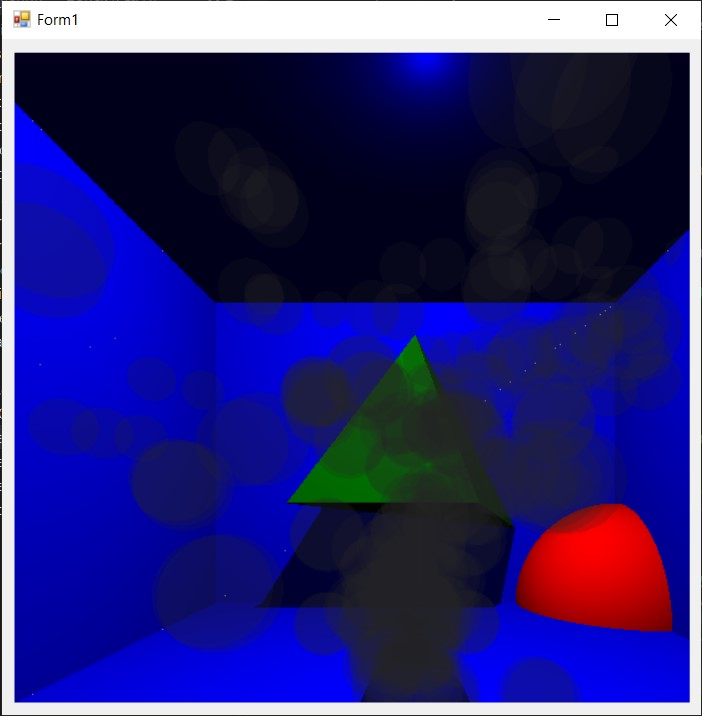
\includegraphics{inc/img/smoke}
	\caption{Демонстрация работы программы в графическом интерфейсе с дымом}
	\label{fig:smoke}
\end{figure}


\begin{figure}[H]
	\centering
	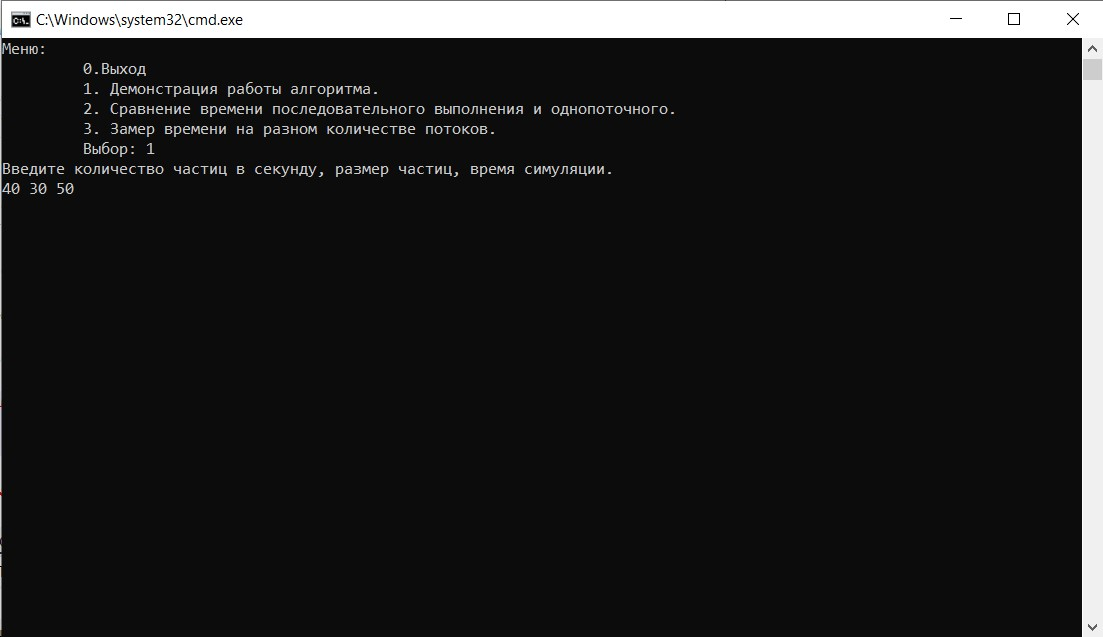
\includegraphics[width=1\linewidth]{inc/img/democonsole}
	\caption{Демонстрация работы программы в консоли}
	\label{fig:democonsole}
\end{figure}


\section{Время выполнения реализаций алгоритмов}

Время выполнения реализаций алгоритмов было замерено при помощи класса Stopwatch \cite{cpplangtime}. 

Замеры времени для каждого количества потоков, каждого количества дополнительных объектов на сцене проводились 50 раз. В качестве результата взято среднее время работы алгоритма на данном количестве потоков, данном количестве дополнительных объектов на сцене.
 
\subsection{Сравнение времени работы реализаций последовательного алгоритма и однопоточного}
Результаты замеров приведены в таблице \ref{tab:single}.
На рисунке \ref{fig:single}, приведен график зависимости времени работы реализаций алгоритмов при последовательном и однопоточном выполнении от количества объектов. Под дополнительными объектами понимаются объекты, добавленные пользователем на сцену после ее создания.

\captionsetup{justification=raggedright,singlelinecheck=false}

\begin{table}[H]
	\begin{center}
		\caption{\label{tab:single}Время выполнения алгоритма обратной трассировки лучей при однопоточном и последовательном выполнении}
		\begin{tabular}{|c|c|c|}
			\hline
			\makecell{Количество\\ дополнительных\\ объектов}&	\makecell{Однопоточное \\выполнение}&	\makecell{Последовательное\\ выполнение} \\ [4ex]
			\hline
			0&	4284,38&	3973,45\\
			\hline
			100&	15784,67&	14135,63\\
			\hline
			200&	26939,55&	24102,88\\
			\hline
			300&	37635,08&	33852,40\\
			\hline
			400&	48896,23&	43472,16\\
			\hline
		\end{tabular}
	\end{center}
\end{table}
\captionsetup{justification=centering,singlelinecheck=false}
\begin{figure}[H]
	\centering
	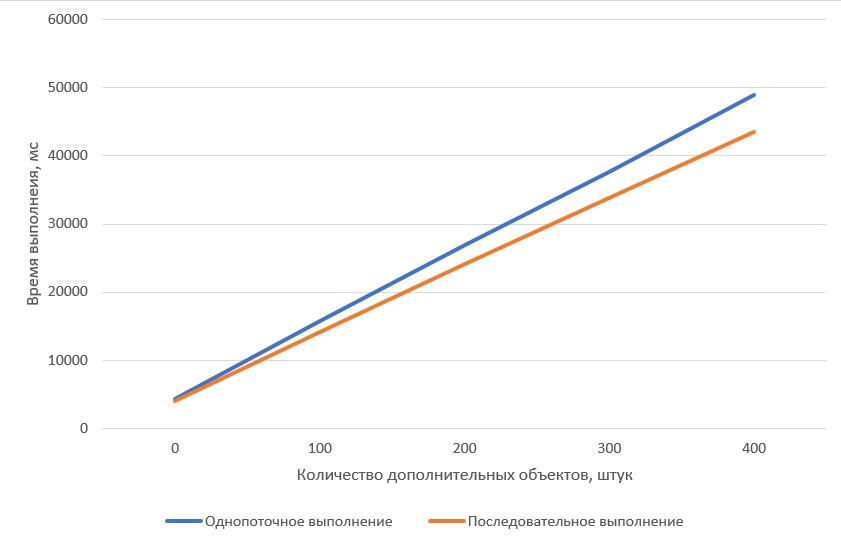
\includegraphics{inc/img/single_fig}
	\caption{Зависимость времени выполнения реализации алгоритма обратной трассировки лучей при однопоточном  и последовательном выполнении}
	\label{fig:single}
\end{figure}

Обычная реализация работает быстрее, чем многопоточный с одним рабочим потоком, потому что на создание потока тратится некоторое время.

\subsection{Сравнение времени выполнения реализаций на разном количестве потоков и дополнительных объектов сцены}

Результаты замеров приведены в таблице \ref{tab:time}.
На рисунке \ref{fig:compfig} приведена зависимость времени работы реализации параллельного алгоритма от количества потоков и количества дополнительных объектов на сцене.
\captionsetup{justification=raggedright,singlelinecheck=false}
\begin{table}[H]
	\begin{center}
		\caption{\label{tab:time}Время выполнения реализации алгоритма обратной трассировки лучей при количества потоков и количества дополнительных объектов на сцене}
		\begin{tabular}{|c|c|c|c|c|c|}
			\hline				
			\multirow{3}{*}{\makecell{Количество\\ дополнительных\\ объектов, штук}} & 	\multicolumn{5}{c|}{Количество потоков, штук} \\ [3ex]
			\cline{2-6}		
			&6&	12&	24&	48&	96\\
			\hline		
			0&	1042,34&	846,74&	948,4&	1060,27&	1100,81\\
			\hline		
			100&	4296,44&	3985,65&	4652,67&	5525,89&	8310,33\\
			\hline		
			200&	7452,28&	6961,98&	7774,77&	9657,25&	15114,46\\
			\hline		
			300&	10535,29&	9723,64&	10917,22&	13735,63&	21985,89\\
			\hline		
			400&	13554,05&	12617,40&	14056,36&	17697,46&	28090,16\\
			\hline		
			500&	16598,27&	15430,81&	17155,82&	21554,69&	34441,75\\
			\hline		
			600&	19478,49&	18153,36&	20216,83&	25357,24&	40506,90\\
			\hline		
			700&	22439,01&	20859,34&	23142,67&	28801,52&	46301,25\\
			\hline		
			800&	25183,41&	23443,41&	26192,44&	32830,08&	51871,79\\
			\hline		
			
		\end{tabular}
	\end{center}
\end{table}
\captionsetup{justification=centering,singlelinecheck=false}
\begin{figure}[H]
	\centering
	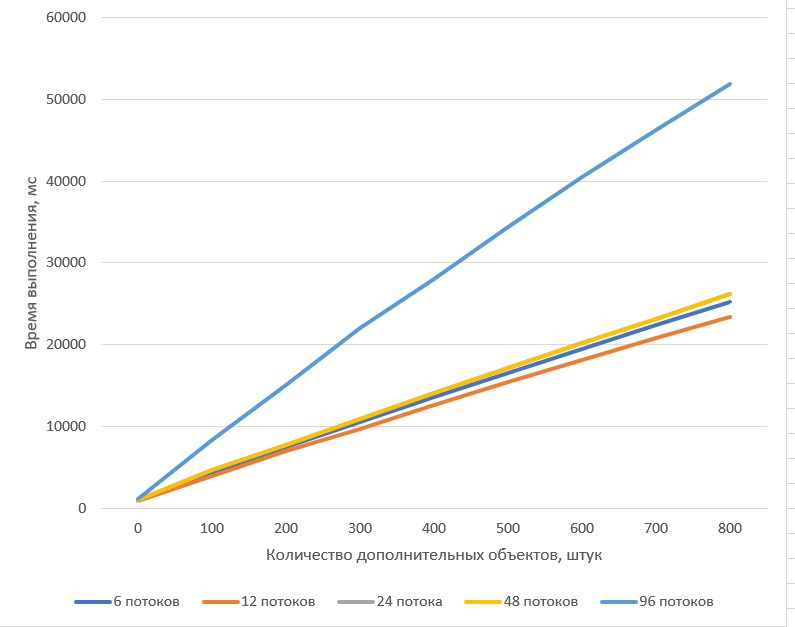
\includegraphics{inc/img/comp_fig}
	\caption{Зависимость времени выполнения реализации алгоритма обратной трассировки лучей от количества потоков и количества дополнительных объектов на сцене}
	\label{fig:compfig}
\end{figure}

При 12 потоках достигается пик, при котором все логические ядра процессора одновременно выполняют трассировку лучей. Далее при увеличении числа потоков производительность падает. Это объясняется тем, что создается очередь потоков, которая замедляет работу программы.

\section*{Вывод}

В данном разделе было произведено сравнение времени выполнения реализации алгоритма трассировки лучей при последовательной реализации и многопоточной. Результат показал, что выгоднее всего использовать столько потоков, сколько у процессора логических ядер.

